\chapter{Speed Detection}
\label{chap:speed-detection}

One of the most important features of the speedcamera is the possibility to measure the speed of objects using only a video feed. The measurement of 
speed can be accomplished using for example AI or multi-camera systems. This chapter shows all the accumulated research about the speed measurement 
and detection. The list below shows some of the basic requirements to ensure accurate speed calculations.

\begin{itemize}
    \item Know distance between stationary (or generated) objects in video;
    \item Camera positioning (90 degree angle, if not possible use image processing);
    \item Solid frame-rate (basic requirement for accurate calculations), with a minimum of 30 fps.
\end{itemize}

\section{Camera-only speed measuring method}
It is possible to create a system using a multi-camera based solution to measure vehicle speed. This can be achieved using for example two cameras,
which are positioned to record two sections of the same road. A vehicle is digitally recorded as they pass through a cameras recording area, this data
is then used to calculate the average speed of the vehicle using the data from both cameras. See figure \ref{fig:two_camera_measurement_overview} for 
an overview of this possible solution.

\begin{linfigure}{fig:two_camera_measurement_overview}{Overall view of the two-camera based vehicle speed measurement.}
    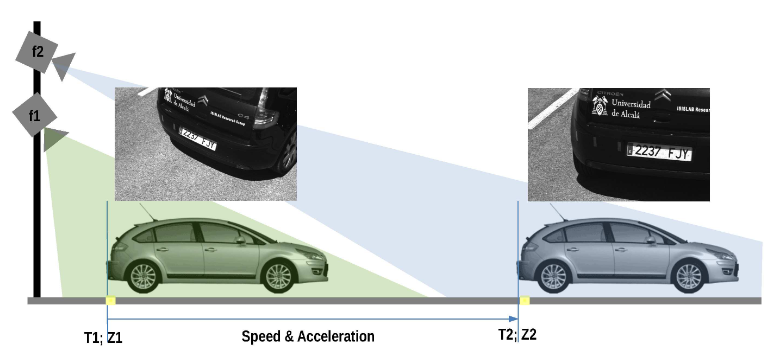
\includegraphics[width=0.75\textwidth]{Two_camera_measurement_overall_view}
\end{linfigure}

As seen in figure \ref{fig:two_camera_measurement_overview} two cameras are used to record a fixed point on the road. These cameras are setup using a
fixed pole in the road. However, this setup can also be achieved using smaller constructions allowing for a clearer view of a licence plate. Using 
this setup allows for use of vision-type programming and a more linear way of licence plate recognition. Experiments have also shown that using the 
setup shown in figure \ref{fig:two_camera_measurement_overview} has a base a maximum speed error of less then 3kmh, meaning it is conform the given
requirements by the client. 

\section{VASCAR speed measuring method}
A VASCAR is a device/technique containing a stopwatch and a processor. The VASCAR starts recording time when a vehicle passes a fixed/generated spot 
on the road, after the vehicle has passed another predetermined fixed/generated spot the recording will stop. The vehicles average speed is then calculated 
by distance between points and the time taken for the vehicle to pass over them. 

Due to radar and LIDAR techniques being illegal and not being allowed by the client, the VASCAR method is a viable option due to it not relying on 
these two methods.

The camera does not have to be in line with the road, due to it being focused on a singular/dual point on the road. And it uses the following formula:
\begin{equation}
    speed = distance \div time
\end{equation}


If the formula 5.1 does not work conform the measurement requirements, the following formulas can be used to calculate the average speed of an object:
\begin{equation}
    Meters Per Pixel = mmp = Distance Constant \div Frame Width
\end{equation}
\begin{equation}
    Distance In Pixels = p_{ab} = | col_A - col_B |
\end{equation}
\begin{equation}
    Distance In Meters Zone_{ab} = d_{ab} = p_{ab} \times mmp
\end{equation}
\begin{equation}
    Average Speed = \Delta d_{ab} \div t_{ab}
\end{equation}

\subsection{Object tracking}
The cameras FOV can be used as beginning and end points for speed measurements, meaning you start measuring object as soon as they are visible on the 
camera. This also allows the device to measure the speed of objects from left-to-right and right-to-left. An object detector and centroid tracker are 
a possibility for this approach, using OpenCV. See LINK TO LICENCE RECOGNITION for research about an AI or algorithm to realize this.

A centroid tracker can be used to track the center of an object, and to use this to measure time required to pass through the cameras view. An example 
of centroid tracking can be seen in figure 1.

\begin{linfigure}{fig:centroid_example}{Example of how centroid tracking works.}
    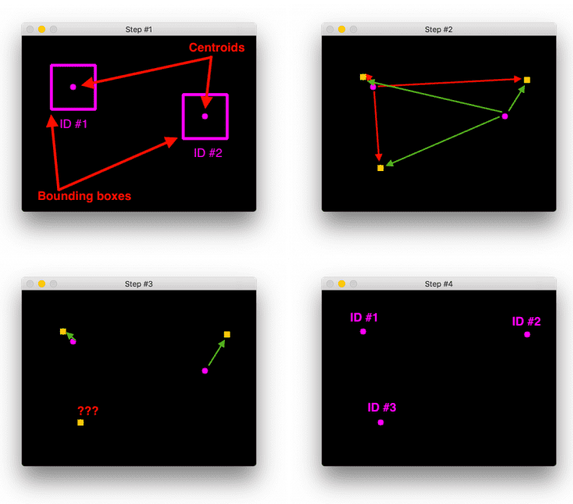
\includegraphics[width=0.75\textwidth]{Centroid_tracking_example}
\end{linfigure}

\begin{lintable}{tbl:steps_in_centroid_example}{Steps displayed in figure \ref{fig:centroid_example}}
    \begin{lintabular}{l|l}
        \lintablehead{Step & Step description}
        \lintablerow{1 & Accept bounding box coordinated and calculate the center of objects. (First frame with existing object)}
        \lintablerow{2 & Calculate distance between new bounding boxes and existing objects. (Frame where a new object is detected)}
        \lintablerow{3 & Update x,y-coordinates of existing objects. (One unknown due to new object)}
        \lintablerow{4 & Register new objects and deregister old objects.}
    \end{lintabular}
\end{lintable}

\newpage

\section{Speed measurement using licence plate recognition}
It is possible to use the position and size of a car's license plate to measure its speed. This requires a very solid license plate detection 
algorithm, which makes it a bit more difficult to use. However, it is very possible if the license plate detection is very reliable, see
figure \ref{fig:license_plate_speed_detection} for an example of this speed measurement method. Furthermore, this method of measuring speed
can be vision-based, meaning this method does not require the use of AI, though it is still optional.

\begin{linfigure}{fig:license_plate_speed_detection}{Overview of the license plate speed measurement method.}
    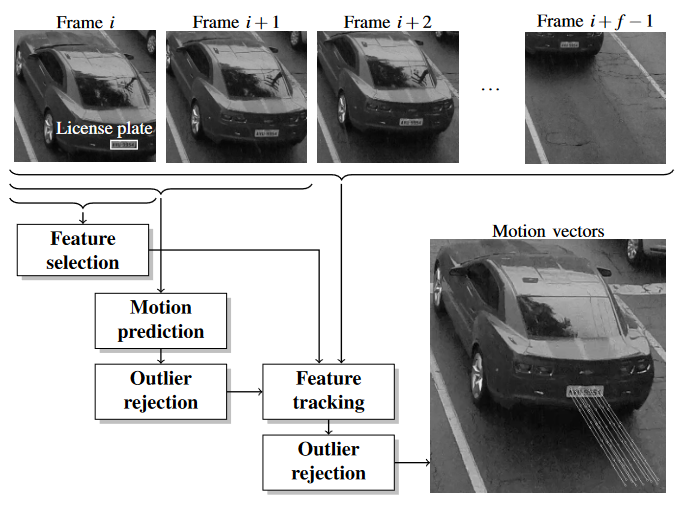
\includegraphics[width=0.75\textwidth]{License_plate_speed_measurement_example}
\end{linfigure}
